%%%%%%%%%%%%%%%%%%%%%%%%%%%%%%%%%%%%%%%%%%%%%%%%%%%
%% LaTeX book template                           %%
%% Author:  Amber Jain (http://amberj.devio.us/) %%
%% License: ISC license                          %%
%%%%%%%%%%%%%%%%%%%%%%%%%%%%%%%%%%%%%%%%%%%%%%%%%%%

\documentclass[a4paper,11pt,fleqn]{book}
\usepackage[a4paper, total={7.5in, 8in}]{geometry}
\usepackage[T1]{fontenc}
\usepackage[utf8]{inputenc}
\usepackage{lmodern}
\usepackage{listings}
\lstset{basicstyle=\ttfamily,
  showstringspaces=false,
  commentstyle=\color{red},
  keywordstyle=\color{blue}
}
\lstset{escapeinside={<@}{@>}}
\usepackage{alltt}
\usepackage{fancyvrb}
\usepackage{cite}
\usepackage[dvipsnames]{xcolor}
\setlength{\parindent}{0pt} % avoids indentation
%%%%%%%%%%%%%%%%%%%%%%%%%%%%%%%%%%%%%%%%%%%%%%%%%%%%%%%%%
% Source: http://en.wikibooks.org/wiki/LaTeX/Hyperlinks %
%%%%%%%%%%%%%%%%%%%%%%%%%%%%%%%%%%%%%%%%%%%%%%%%%%%%%%%%%
\usepackage{hyperref}
\usepackage{caption}
\captionsetup{justification=raggedright,singlelinecheck=false}
\usepackage{graphicx}
\usepackage[english]{babel}
\usepackage{amsmath}
\usepackage{mathtools}
\usepackage{xcolor}
\usepackage{breqn}   % Breaks the equations into linea automatically
\usepackage{amsmath} % Breaks the equations into lines manually putting ``//''
%%%%%%%%%%%%%%%%%%%%%%%%%%%%%%
% Tikz
%%%%%%%%%%%%%%%%%%%%%%%%%%%%%%
\usepackage{standalone}
\usepackage{tikz}
\usetikzlibrary{matrix,backgrounds,calc,shapes,arrows,fit,positioning} % Tikz libraries required for the flow chart in the template
\usetikzlibrary{chains,shapes.multipart}
\usetikzlibrary{shapes,calc}
\usetikzlibrary{automata,positioning}
\usepackage{forest}
%%%%%%%%%%%%%%%%%%%%%%%%%%%%%%%%%%%%%%%%%%%%%%%%%%%%%%%%%%%%%%%%%%%%%%%%%%%%%%%%
% 'dedication' environment: To add a dedication paragraph at the start of book %
% Source: http://www.tug.org/pipermail/texhax/2010-June/015184.html            %
%%%%%%%%%%%%%%%%%%%%%%%%%%%%%%%%%%%%%%%%%%%%%%%%%%%%%%%%%%%%%%%%%%%%%%%%%%%%%%%%
\newenvironment{dedication}
{
   \cleardoublepage
   \thispagestyle{empty}
   \vspace*{\stretch{1}}
   \hfill\begin{minipage}[t]{0.66\textwidth}
   \raggedright
}
{
   \end{minipage}
   \vspace*{\stretch{3}}
   \clearpage
}

%%%%%%%%%%%%%%%%%%%%%%%%%%%%%%%%%%%%%%%%%%%%%%%%
% Chapter quote at the start of chapter        %
% Source: http://tex.stackexchange.com/a/53380 %
%%%%%%%%%%%%%%%%%%%%%%%%%%%%%%%%%%%%%%%%%%%%%%%%
\makeatletter
\renewcommand{\@chapapp}{}% Not necessary...
\newenvironment{chapquote}[2][2em]
  {\setlength{\@tempdima}{#1}
   \def\chapquote@author{#2}%
   \parshape 1 \@tempdima \dimexpr\textwidth-2\@tempdima\relax%
   \itshape}
  {\par\normalfont\hfill--\ \chapquote@author\hspace*{\@tempdima}\par\bigskip}
\makeatother

\newcommand{\sputnik}{\texttt{SPUTNIK }}
\newcommand{\macro}{\texttt{MACRO }}
\newcommand{\micro}{\texttt{MICRO }}
\newcommand{\micflag}{\texttt{mic\_flag }}
\newcommand{\gmsh}{\texttt{Gmsh }}
\newcommand{\parmetis}{\texttt{ParMetis }}
%%%%%%%%%%%%%%%%%%%%%%%%%%%%%%%%%%%%%%%%%%%%%%%%%%%
% First page of book which contains 'stuff' like: %
%  - Book title, subtitle                         %
%  - Book author name                             %
%%%%%%%%%%%%%%%%%%%%%%%%%%%%%%%%%%%%%%%%%%%%%%%%%%%

% Book's title and subtitle
\title{\Huge \textbf{SPUTNIK}\\ \huge Code for multi-scale calculations on solids. }
% Author
\author{\textsc{Guido Giuntoli}}

% Images path
\graphicspath{{images/}}

\begin{document}

\frontmatter
\maketitle

%%%%%%%%%%%%%%%%%%%%%%%%%%%%%%%%%%%%%%%%%%%%%%%%%%%%%%%%%%%%%%%
% Add a dedication paragraph to dedicate your book to someone %
%%%%%%%%%%%%%%%%%%%%%%%%%%%%%%%%%%%%%%%%%%%%%%%%%%%%%%%%%%%%%%%

\begin{dedication}
Dedicated to my mum Patricia, dad Miguel, sister Julia and dog Jenny.
\end{dedication}

%%%%%%%%%%%%%%%%%%%%%%%%%%%%%%%%%%%%%%%%%%%%%%%%%%%%%%%%%%%%%%%%%%%%%%%%
% Auto-generated table of contents, list of figures and list of tables %
%%%%%%%%%%%%%%%%%%%%%%%%%%%%%%%%%%%%%%%%%%%%%%%%%%%%%%%%%%%%%%%%%%%%%%%%
\tableofcontents
% \listoffigures
% \listoftables

\mainmatter

%%%%%%%%%%%
% Preface %
%%%%%%%%%%%
% \chapter*{Preface}

\par
\sputnik is code for calculating a composite material structure. It is composed by two main codes called \macro and
\micro each one design for perfomed coupled calculation with themselves.




%%%%%%%%%%%%%%%%%%%%%%%%%%%%%%%%%%%%
% Give credit where credit is due. %
% Say thanks!                      %
%%%%%%%%%%%%%%%%%%%%%%%%%%%%%%%%%%%%
% \section*{Acknowledgements}
% \begin{itemize}
% \item A special word of thanks goes to Professor Don Knuth\footnote{\url{http://www-cs-faculty.stanford.edu/~uno/}} (for \TeX{}) and Leslie Lamport\footnote{\url{http://www.lamport.org/}} (for \LaTeX{}).
% \item I'll also like to thank Gummi\footnote{\url{http://gummi.midnightcoding.org/}} developers and LaTeXila\footnote{\url{http://projects.gnome.org/latexila/}} development team for their awesome \LaTeX{} editors.
% \item I'm deeply indebted my parents, colleagues and friends for their support and encouragement.
% \end{itemize}
% \mbox{}\\
% %\mbox{}\\
% \noindent Amber Jain \\
% \noindent \url{http://amberj.devio.us/}

%%%%%%%%%%%%%%%%
% CHAPTERS %
%%%%%%%%%%%%%%%%
\chapter*{Preface}

\par
\sputnik is code for calculating a composite material structure. It is composed by two main codes called \macro and
\micro each one design for perfomed coupled calculation with themselves.



\chapter{Code design}

\section{Introduction}

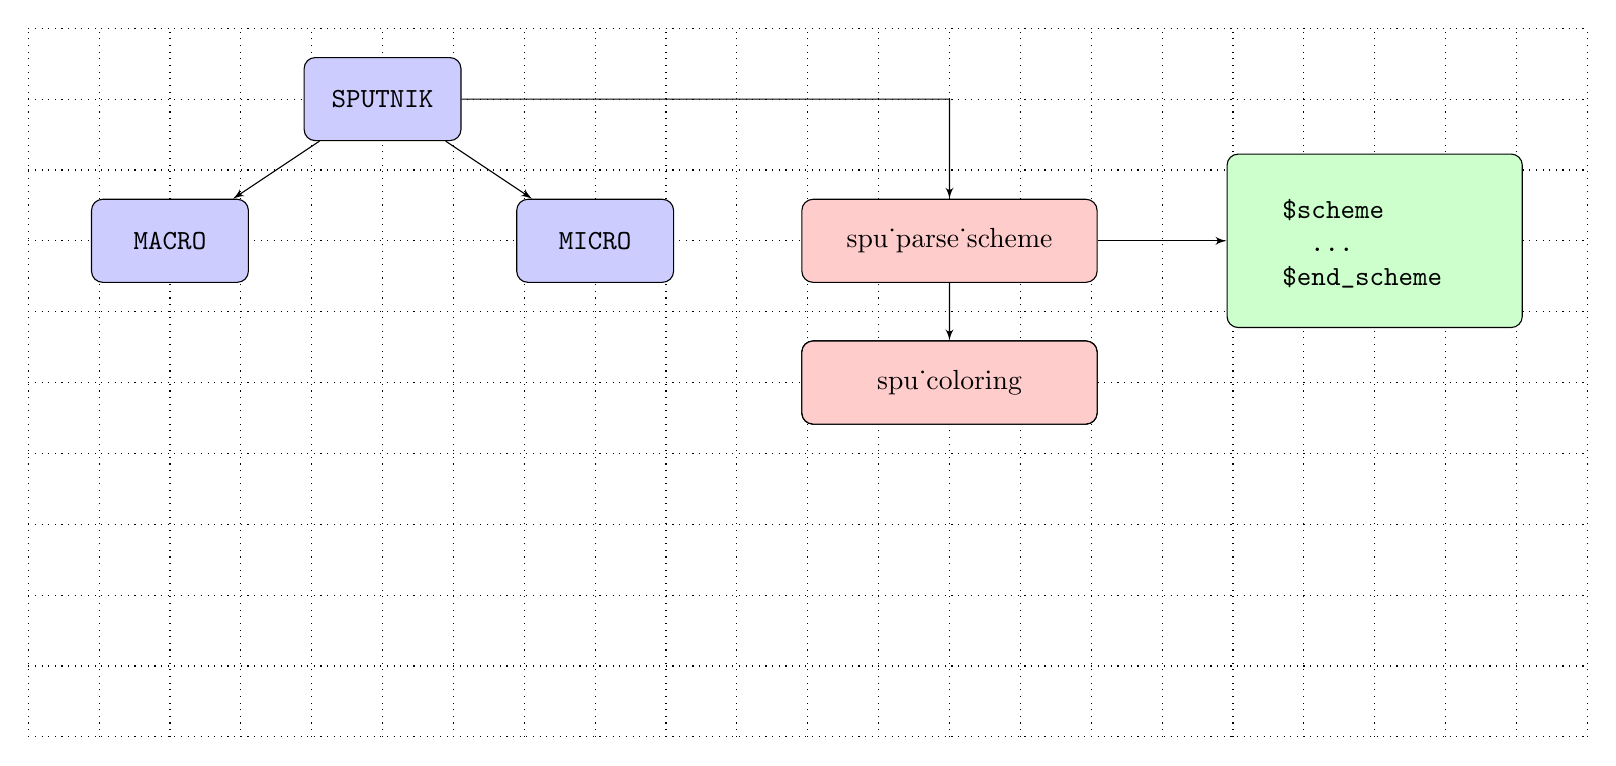
\begin{tikzpicture}[scale=0.9,node distance = 2cm, auto]

   \tikzstyle{block}  = [rectangle, draw, fill=blue!20 , text width=5em, text centered, rounded corners, minimum height=3em]
   \tikzstyle{blockf} = [rectangle, draw, fill=red!20  , text width=10em, text centered, rounded corners, minimum height=3em]
   \tikzstyle{blockc} = [rectangle, draw, fill=green!20, text width=10em, text centered, rounded corners, minimum height=3em]
   \tikzstyle{line}   = [draw, -latex']
   \tikzstyle{blocke} = [rectangle, draw, text width=9em, text centered, rounded corners, minimum height=2.5em]

   % draw a grid for positioning nodes
   \coordinate (bottom_left) at (0,0);
   \coordinate (top_right) at (22,10);
   \draw [dotted, draw=black, fill=white] (bottom_left) grid  (top_right);

   \node [block] (sput) at (5,9)  {\sputnik};
   \node [block] (macr) at (2,7)  {\macro};
   \node [block] (micr) at (8,7) {\micro};
   \node [blockf] (pars) at (13,7) {spu_parse_scheme};
   \node [blockc] (parc) at (19,7) {
     \begin{verbatim}
     $scheme
        ...
     $end_scheme
     \end{verbatim}
     };

   \node [blockf] (colo) at (13,5) {spu_coloring};
   \node [blockf] (colo) at (13,5) {spu_coloring};
   \node [blockf] (colo) at (13,5) {spu_coloring};
   
   \path [line] (sput) -- (macr);
   \path [line] (sput) -- (micr);
   \path [line] (sput) -- (13,9) -- (pars);
   \path [line] (pars) -- (colo);
   \path [line] (pars) -- (parc);
   %\draw [->,line width=2] (thermo)  to[bend left,outer ysep=1em] node {$\sigma$} (coupvol) ;

\end{tikzpicture}

%%%%%%%%%%%%%%%%%%%%%%%%%%%%%%%%%%%%%%%%%%%%%%%%%%%%%%%%%%%%%

\section{\sputnik Data-structures}

In the code exist an array \texttt{id_vec} that in each position \texttt{i} has the \texttt{id} of the code that is
executing (\texttt{id = MACRO|MICRO}). For obtaining this array an \texttt{MPI_Allgather} operation is performed. Using
this array at the it is possible to check is the options on the input file have sense.


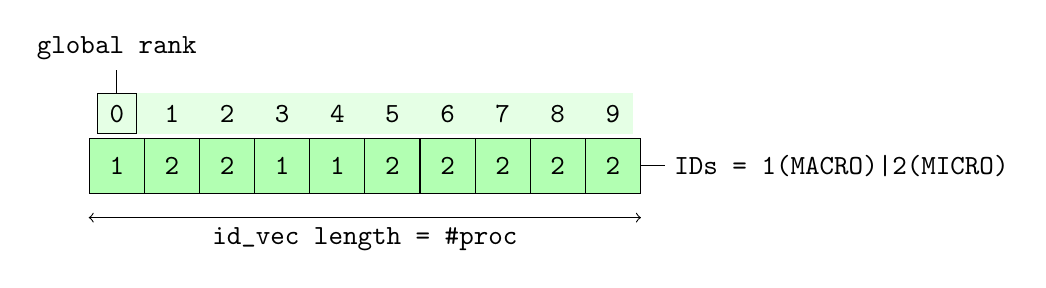
\begin{tikzpicture}[font=\ttfamily,
array/.style={matrix of nodes,nodes={draw, minimum size=7mm, fill=green!30},column sep=-\pgflinewidth, row sep=0.5mm, nodes in empty cells,
row 1/.style={nodes={draw=none, fill=none, minimum size=5mm}},
row 1 column 1/.style={nodes={draw}}}]

    \matrix[array] (array) {
        0 & 1 & 2 & 3 & 4 & 5 & 6 & 7 & 8 & 9\\
        1 & 2 & 2 & 1 & 1 & 2 & 2 & 2 & 2 & 2\\};
    %\node[draw, fill=gray, minimum size=4mm] at (array-2-9) (box) {};

    \begin{scope}[on background layer]
    \fill[green!10] (array-1-1.north west) rectangle (array-1-10.south east);
    \end{scope}

    \draw[<->]([yshift=-3mm]array-2-1.south west) -- node[below] {id_vec length = \#proc} ([yshift=-3mm]array-2-10.south east);

    \draw (array-1-1.north)--++(90:3mm) node [above] (first) {global rank};
    \draw (array-2-10.east)--++(0:3mm) node [right]{IDs = 1(MACRO)|2(MICRO)};
    %\node [align=center, anchor=south] at (array-2-9.north west|-first.south) (8) {IDs\\ MACRO=1 MICRO=1};
    %\draw (8)--(box);
    %
\end{tikzpicture}

%%%%%%%%%%%%%%%%%%%%%%%%%%%%%%%%%%%%%%%%%%%%%%%%%%%%%%%%%%%%%

\section{\sputnik Communication Approaches}

\subsection{\texttt{Scheme 2}}

All the macro-processes communicates with the same micro-processes. In this approach is possible to parallelize the
assembling process doing calculations on both micro-structures at the same time.

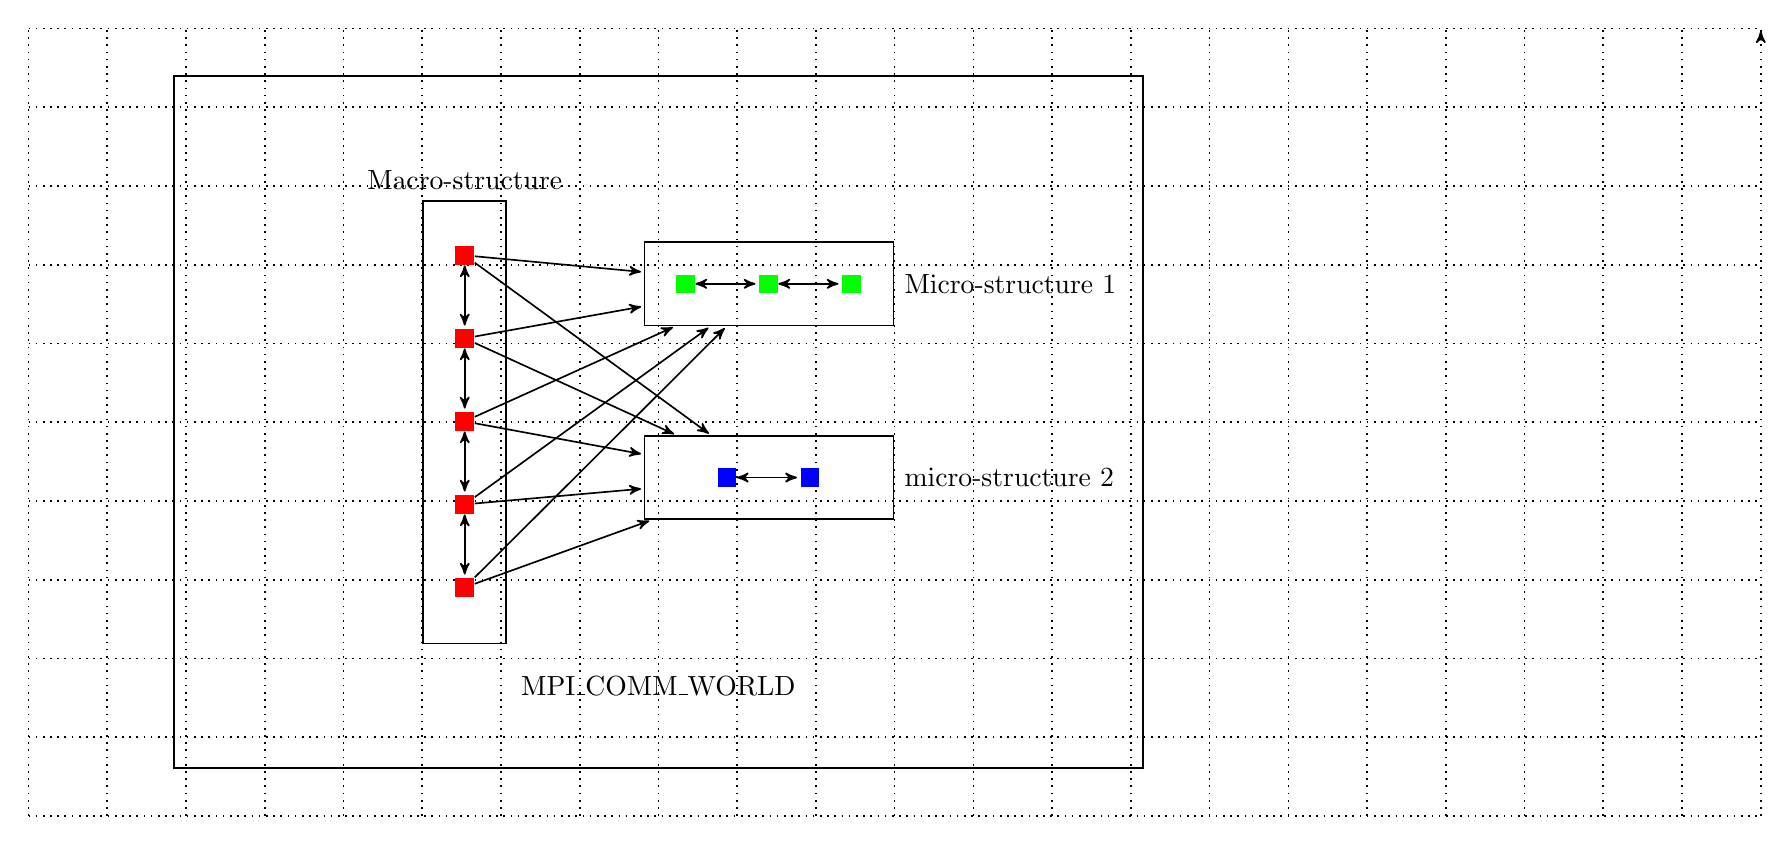
\begin{tikzpicture}[->,>=stealth',shorten >=1pt,auto,node distance=3em,semithick]

   \tikzstyle{state} =[fill=red,draw=none,text=white,minimum size=0.1cm]
   \tikzstyle{type2}=[fill=green,draw=none,text=white,minimum size=0.1cm]
   \tikzstyle{type3}=[fill=blue,draw=none,text=white,minimum size=0.1cm]

   % draw a grid for positioning nodes
   \coordinate (bottom_left) at (0,0);
   \coordinate (top_right) at (22,10);
   \draw [dotted, draw=black, fill=white] (bottom_left) grid  (top_right);

    \node[draw,minimum width=35em,minimum height=25em,font=\small,label={[xshift=0.0cm, yshift=-8.0cm]
  	MPI\_COMM\_WORLD} ]  at (8,5) (world){} ;
  
    \node[draw,minimum width=3em,minimum height=16em,font=\small, label=above:{Macro-structure}] 
    at ([xshift=-7em]world.center) (macro){};
  
    \node[draw,minimum width=9em,minimum height=3em,font=\small, label=right:{Micro-structure 1}] 
    at ([xshift=+4em,yshift=+5em]world.center) (micro1){} ;
  
    \node[draw,minimum width=9em,minimum height=3em,font=\small, label=right:{micro-structure 2}] 
    at ([xshift=+4em,yshift=-2em]world.center) (micro2){} ;
  
  
    \node[state] (A) at ([yshift=-2em]macro.north) {};
    \node[state] (B) [below of=A] {};
    \node[state] (C) [below of=B] {};
    \node[state] (D) [below of=C] {};
    \node[state] (E) [below of=D] {};
  
    \node[type2] (f) at ([xshift=+1.5em]micro1.west) {};
    \node[type2] (g) [right of=f] {};
    \node[type2] (h) [right of=g] {};
  
    \node[type3] (i) at ([xshift=+3em]micro2.west) {};
    \node[type3] (j) [right of=i] {};
  
    \draw [<->] (A) -- (B);
    \draw [<->] (B) -- (C);
    \draw [<->] (C) -- (D);
    \draw [<->] (D) -- (E);
  
    \draw [<->] (f) -- (g);
    \draw [<->] (g) -- (h);

    \draw [<->] (i) -- (j);
  
    \path (A) edge node {} (micro1)
          (B) edge node {} (micro1)
          (C) edge node {} (micro1)
          (D) edge node {} (micro1)
          (E) edge node {} (micro1);

    \path (A) edge node {} (micro2)
          (B) edge node {} (micro2)
          (C) edge node {} (micro2)
          (D) edge node {} (micro2)
          (E) edge node {} (micro2);
  
\end{tikzpicture}

%%%%%%%%%%%%%%%%%%%%%%%%%%%%%%%%%%%%%%%%%%%%%%%%%%%%%%%%%%%%%

\subsection{\texttt{Scheme 2}}

All the macro-processes communicates with all the micro-processes. In this approach is possible to parallelize the
assembling process doing calculations on all micro-structures at the same time. The \emph{scheme}

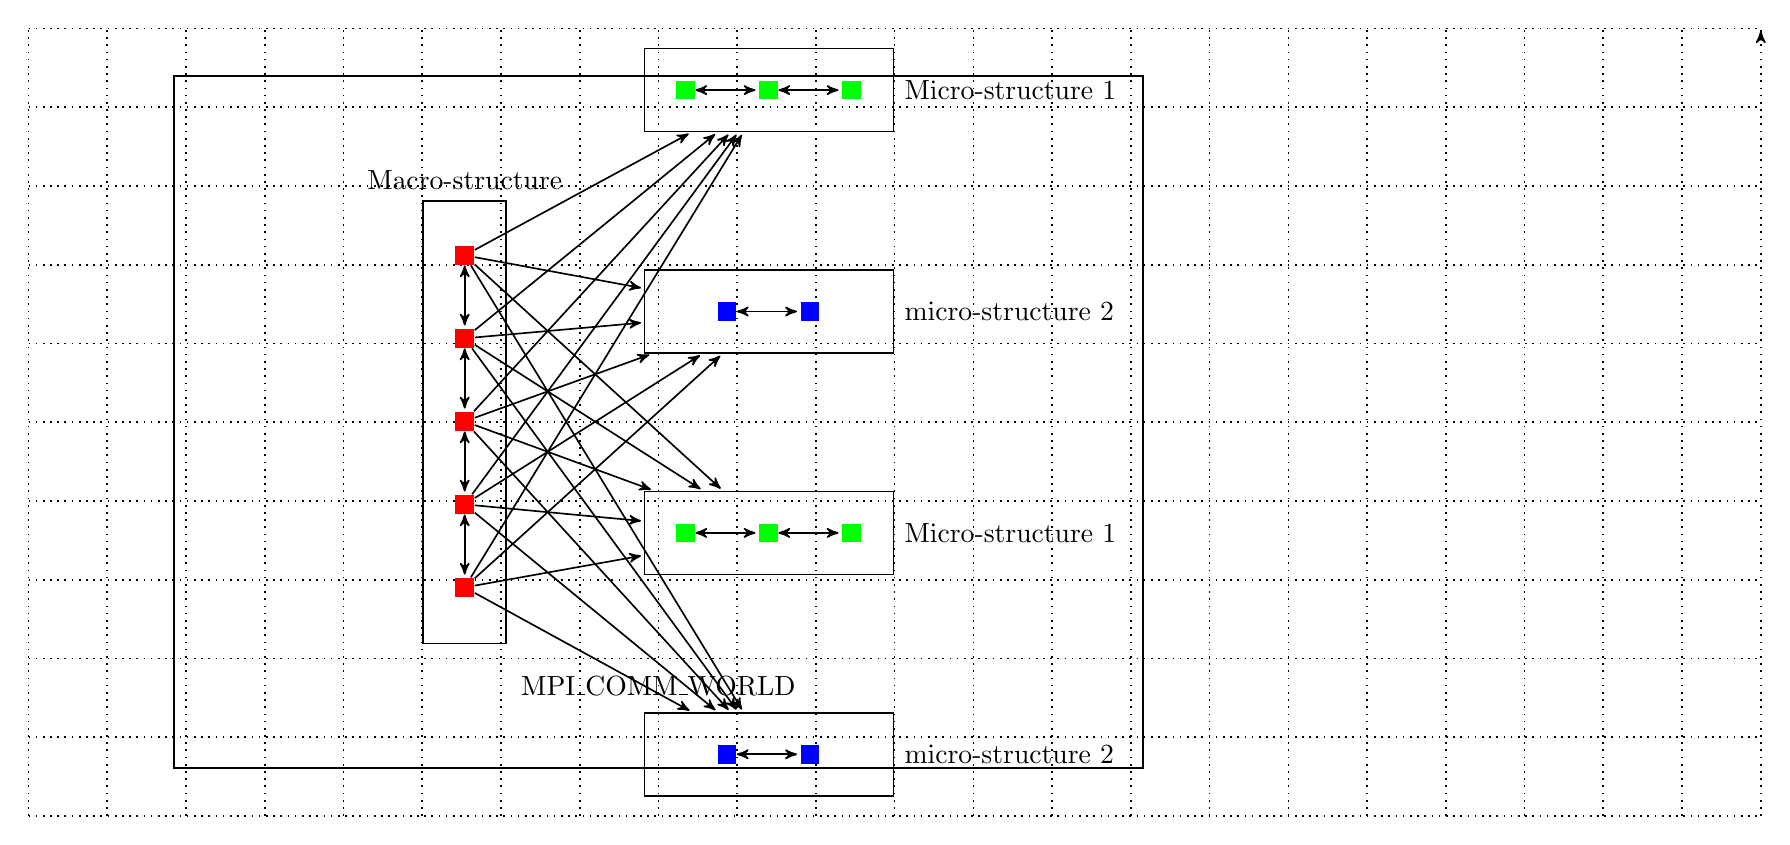
\begin{tikzpicture}[->,>=stealth',shorten >=1pt,auto,node distance=3em,semithick]

   \tikzstyle{state} =[fill=red,draw=none,text=white,minimum size=0.1cm]
   \tikzstyle{type2}=[fill=green,draw=none,text=white,minimum size=0.1cm]
   \tikzstyle{type3}=[fill=blue,draw=none,text=white,minimum size=0.1cm]

   % draw a grid for positioning nodes
   \coordinate (bottom_left) at (0,0);
   \coordinate (top_right) at (22,10);
   \draw [dotted, draw=black, fill=white] (bottom_left) grid  (top_right);

    \node[draw,minimum width=35em,minimum height=25em,font=\small,label={[xshift=0.0cm, yshift=-8.0cm]
  	MPI\_COMM\_WORLD} ]  at (8,5) (world){} ;
  
    \node[draw,minimum width=3em,minimum height=16em,font=\small, label=above:{Macro-structure}] 
    at ([xshift=-7em]world.center) (macro){};
  
    \node[draw,minimum width=9em,minimum height=3em,font=\small, label=right:{Micro-structure 1}] 
    at ([xshift=+4em,yshift=+12em]world.center) (micro1){} ;
  
    \node[draw,minimum width=9em,minimum height=3em,font=\small, label=right:{micro-structure 2}] 
    at ([xshift=+4em,yshift=+4em]world.center) (micro2){} ;

    \node[draw,minimum width=9em,minimum height=3em,font=\small, label=right:{Micro-structure 1}] 
    at ([xshift=+4em,yshift=-4em]world.center) (micro3){} ;
  
    \node[draw,minimum width=9em,minimum height=3em,font=\small, label=right:{micro-structure 2}] 
    at ([xshift=+4em,yshift=-12em]world.center) (micro4){} ;
  
  
    \node[state] (A) at ([yshift=-2em]macro.north) {};
    \node[state] (B) [below of=A] {};
    \node[state] (C) [below of=B] {};
    \node[state] (D) [below of=C] {};
    \node[state] (E) [below of=D] {};
  
    \node[type2] (f) at ([xshift=+1.5em]micro1.west) {};
    \node[type2] (g) [right of=f] {};
    \node[type2] (h) [right of=g] {};
  
    \node[type3] (i) at ([xshift=+3em]micro2.west) {};
    \node[type3] (j) [right of=i] {};
  
    \draw [<->] (A) -- (B);
    \draw [<->] (B) -- (C);
    \draw [<->] (C) -- (D);
    \draw [<->] (D) -- (E);
  
    \draw [<->] (f) -- (g);
    \draw [<->] (g) -- (h);

    \draw [<->] (i) -- (j);
  
    \path (A) edge node {} (micro1)
          (B) edge node {} (micro1)
          (C) edge node {} (micro1)
          (D) edge node {} (micro1)
          (E) edge node {} (micro1);

    \path (A) edge node {} (micro2)
          (B) edge node {} (micro2)
          (C) edge node {} (micro2)
          (D) edge node {} (micro2)
          (E) edge node {} (micro2);

  
    \node[type2] (f2) at ([xshift=+1.5em]micro3.west) {};
    \node[type2] (g2) [right of=f2] {};
    \node[type2] (h2) [right of=g2] {};
  
    \node[type3] (i2) at ([xshift=+3em]micro4.west) {};
    \node[type3] (j2) [right of=i2] {};
  
    \draw [<->] (f2) -- (g2);
    \draw [<->] (g2) -- (h2);

    \draw [<->] (i2) -- (j2);

    \path (A) edge node {} (micro3)
          (B) edge node {} (micro3)
          (C) edge node {} (micro3)
          (D) edge node {} (micro3)
          (E) edge node {} (micro3);

    \path (A) edge node {} (micro4)
          (B) edge node {} (micro4)
          (C) edge node {} (micro4)
          (D) edge node {} (micro4)
          (E) edge node {} (micro4);
  
\end{tikzpicture}

%%%%%%%%%%%%%%%%%%%%%%%%%%%%%%%%%%%%%%%%%%%%%%%%%%%%%%%%%%%%%

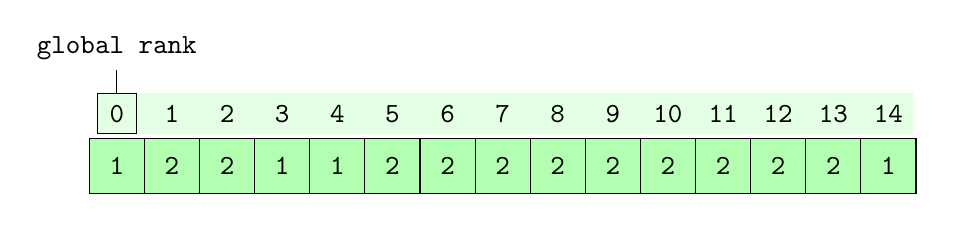
\begin{tikzpicture}[font=\ttfamily,
array/.style={matrix of nodes,nodes={draw, minimum size=7mm, fill=green!30},column sep=-\pgflinewidth, row sep=0.5mm, nodes in empty cells,
row 1/.style={nodes={draw=none, fill=none, minimum size=5mm}},
row 1 column 1/.style={nodes={draw}}}]

    \matrix[array] (array) {
        0 & 1 & 2 & 3 & 4 & 5 & 6 & 7 & 8 & 9 & 10 & 11 & 12 & 13 & 14\\
        1 & 2 & 2 & 1 & 1 & 2 & 2 & 2 & 2 & 2 & 2  & 2  & 2  & 2  & 1\\};
    %\node[draw, fill=gray, minimum size=4mm] at (array-2-9) (box) {};

    \begin{scope}[on background layer]
    \fill[green!10] (array-1-1.north west) rectangle (array-1-15.south east);
    \end{scope}

    %\draw[<->]([yshift=-3mm]array-2-1.south west) -- node[below] {id_vec length = \#proc} ([yshift=-3mm]array-2-10.south east);

    \draw (array-1-1.north)--++(90:3mm) node [above] (first) {global rank};
    %\draw (array-2-10.east)--++(0:3mm) node [right]{IDs = 1(MACRO)|2(MICRO)};
    %\node [align=center, anchor=south] at (array-2-9.north west|-first.south) (8) {IDs\\ MACRO=1 MICRO=1};
    %\draw (8)--(box);
    %
\end{tikzpicture}

%%%%%%%%%%%%%%%%%%%%%%%%%%%%%%%%%%%%%%%%%%%%%%%%%%%%%%%%%%%%%

\section{Mesh treatment}

For both \macro and \micro a mesh reading and partition is performed in order to do parallel operations. The main
characteristics are:

\begin{enumerate}
\item Each process reads a part of the \gmsh file, i.e. a contiguous list of elements acording to his rank. The number
of elements read from each process is more or less the same and can differ at most in one element.
\item A \parmetis function performs the mesh partition giving for each process a \texttt{part} vector whose component
\texttt{e} indicates to which process that element \texttt{e} belongs. 
\item Each part of the mesh is distributed to each process and all process do the same, this is done with a
\texttt{MPI_Alltoall} operation.
\item Each process has the list of elements that belongs to him and know they have to decide which nodes belong to each
one and the new numeration. For doing this we implement different criteria : 
\begin{itemize}
\item \texttt{P0} owns all the nodes detected in its partition so it does not have any ghost nodes. \texttt{P1} ask
\texttt{P0} for his list of nodes and deletes the ones that are repeated in his list and assign them to the list of
ghost nodes. \texttt{P2} ask the same to \texttt{P1} and \texttt{P0} and performs the same operation and so on.
\end{itemize}
\item Each process counts the number of local nodes and share it with an \texttt{MPI_Allgather} operation with the
others. With the number of nodes per process it is possible to assign a local numeration to each local list of nodes on
each process.
\item Each process sends it list of ghost nodes to a common vector with a \texttt{MPI_Allgather} operation and each
process search if one of this nodes belongs to him, if belong it puts on another vector the new numeration of it. It is
not possible that two process have the same node in this instance.
\end{enumerate}

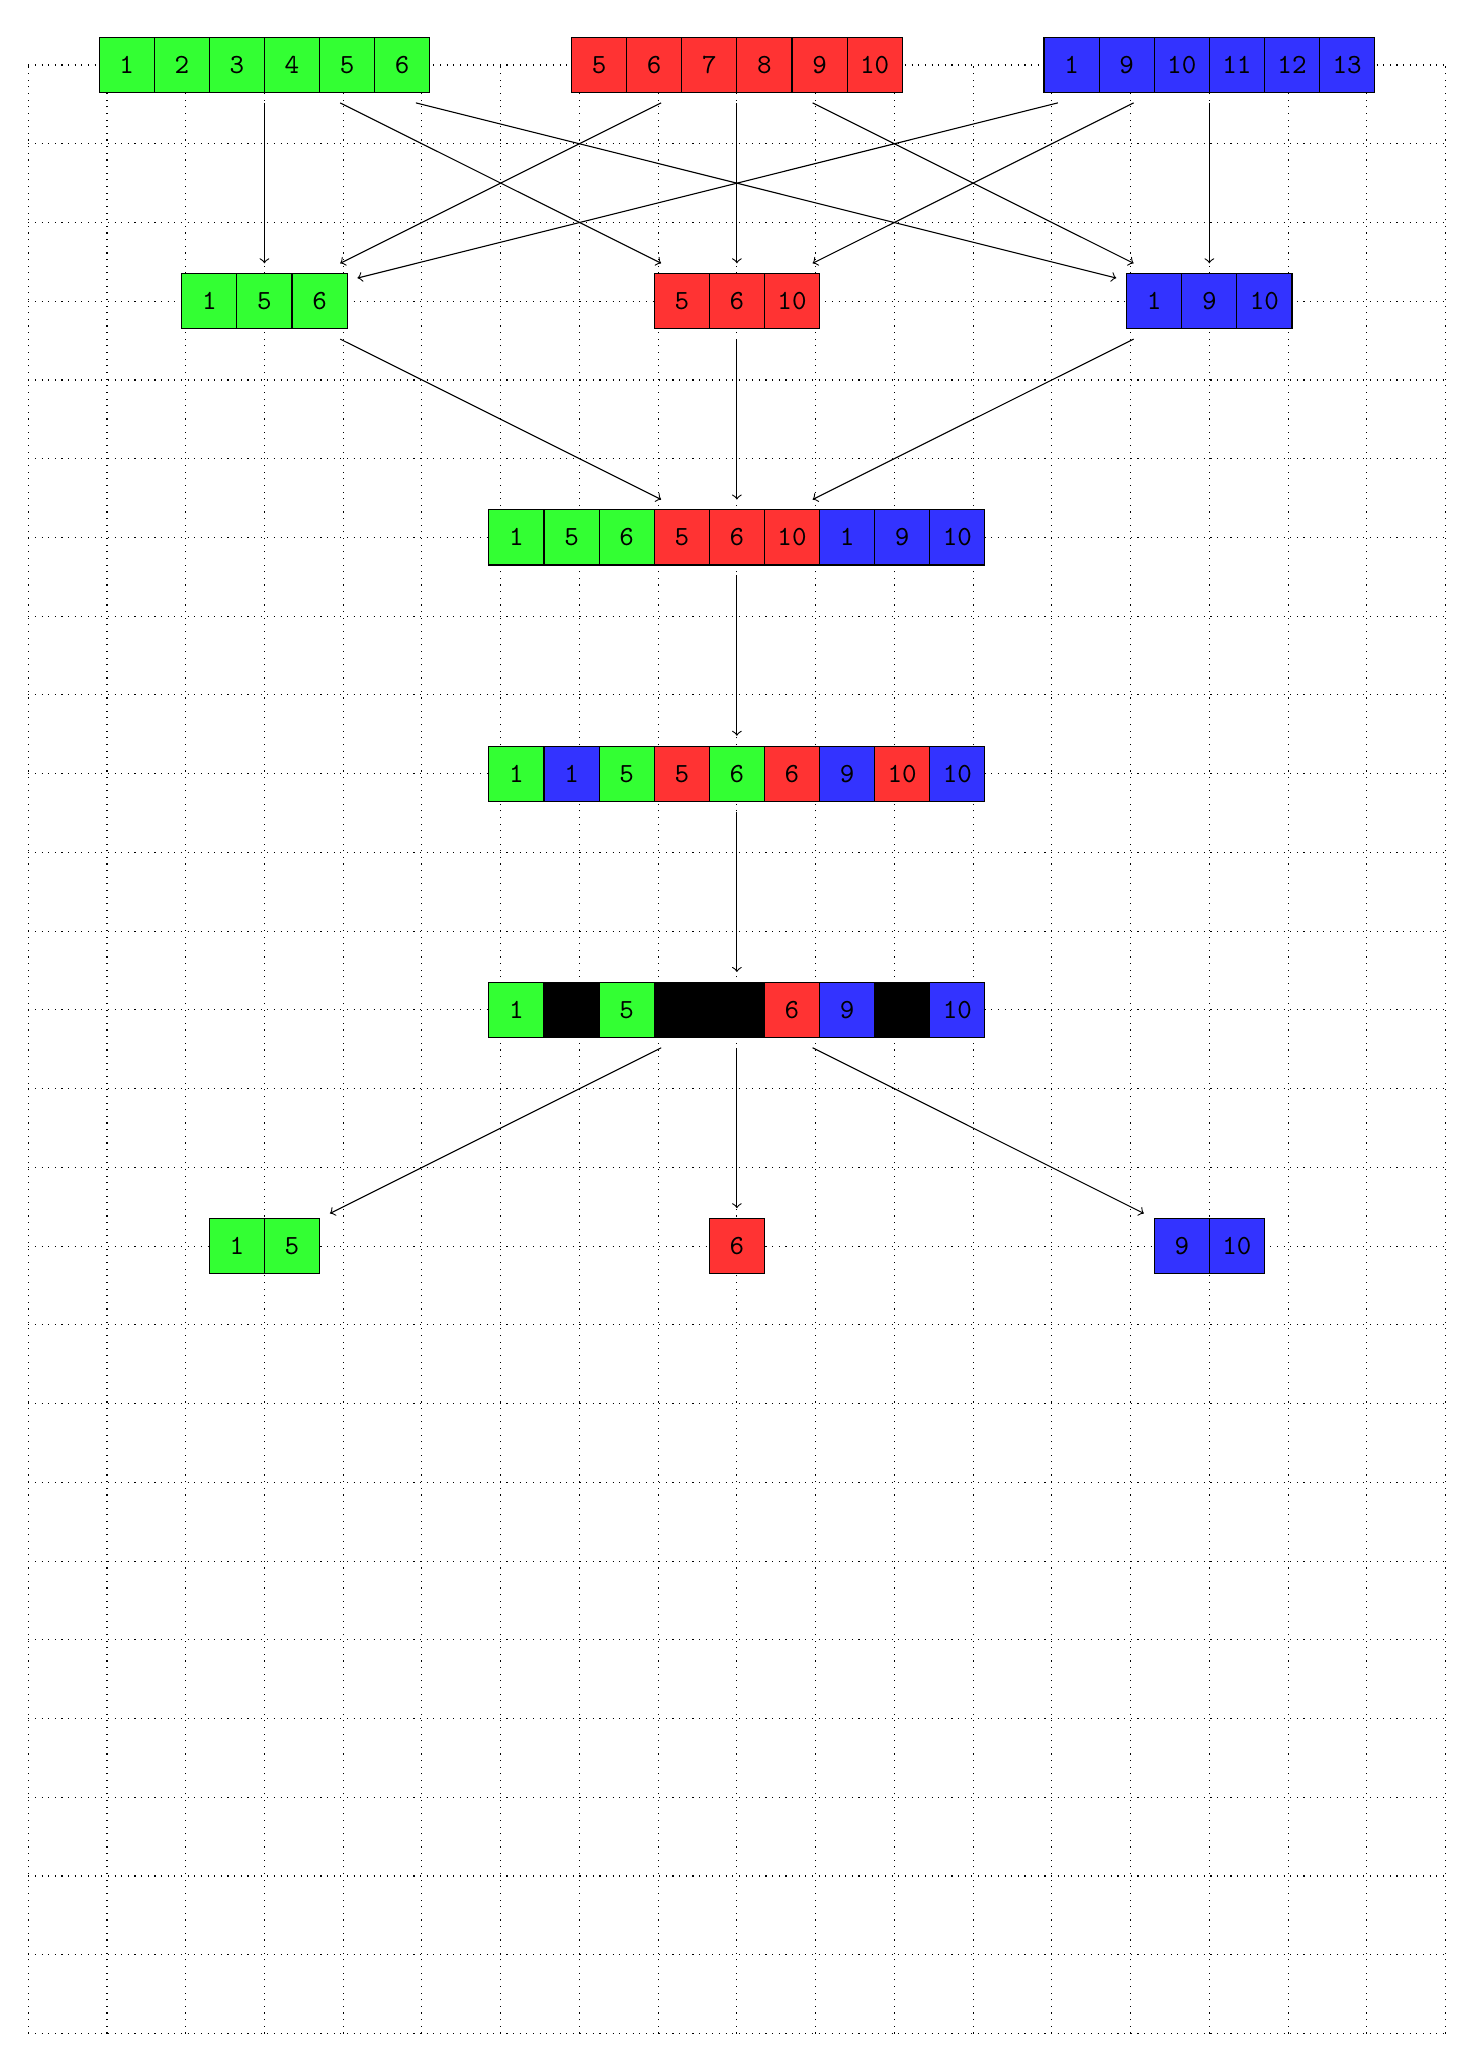
\begin{tikzpicture}[font=\ttfamily,
array_g/.style={matrix of nodes,nodes={draw, minimum size=7mm, fill=green!80},column sep=-\pgflinewidth, row sep=0.5mm, nodes in empty cells,
row 0/.style={nodes={draw=none, fill=none, minimum size=5mm}},
row 0 column 1/.style={nodes={draw}}},
array_r/.style={matrix of nodes,nodes={draw, minimum size=7mm, fill=red!80},column sep=-\pgflinewidth, row sep=0.5mm, nodes in empty cells,
row 0/.style={nodes={draw=none, fill=none, minimum size=5mm}},
row 0 column 1/.style={nodes={draw}}},
array_c/.style={matrix of nodes,nodes={draw, minimum size=7mm, fill=red!100},column sep=-\pgflinewidth, row sep=0.5mm, nodes in empty cells,
row 1 column 1/.style={nodes={draw, fill=green!80}},
row 1 column 2/.style={nodes={draw, fill=green!80}},
row 1 column 3/.style={nodes={draw, fill=green!80}},
row 1 column 4/.style={nodes={draw, fill=red!80}},
row 1 column 5/.style={nodes={draw, fill=red!80}},
row 1 column 6/.style={nodes={draw, fill=red!80}},
row 1 column 7/.style={nodes={draw, fill=blue!80}},
row 1 column 8/.style={nodes={draw, fill=blue!80}},
row 1 column 9/.style={nodes={draw, fill=blue!80}}
},
array_d/.style={matrix of nodes,nodes={draw, minimum size=7mm, fill=red!100},column sep=-\pgflinewidth, row sep=0.5mm, nodes in empty cells,
row 1 column 1/.style={nodes={draw, fill=green!80}},
row 1 column 2/.style={nodes={draw, fill=blue!80}},
row 1 column 3/.style={nodes={draw, fill=green!80}},
row 1 column 4/.style={nodes={draw, fill=red!80}},
row 1 column 5/.style={nodes={draw, fill=green!80}},
row 1 column 6/.style={nodes={draw, fill=red!80}},
row 1 column 7/.style={nodes={draw, fill=blue!80}},
row 1 column 8/.style={nodes={draw, fill=red!80}},
row 1 column 9/.style={nodes={draw, fill=blue!80}}
},
array_d/.style={matrix of nodes,nodes={draw, minimum size=7mm, fill=red!100},column sep=-\pgflinewidth, row sep=0.5mm, nodes in empty cells,
row 1 column 1/.style={nodes={draw, fill=green!80}},
row 1 column 2/.style={nodes={draw, fill=blue!80}},
row 1 column 3/.style={nodes={draw, fill=green!80}},
row 1 column 4/.style={nodes={draw, fill=red!80}},
row 1 column 5/.style={nodes={draw, fill=green!80}},
row 1 column 6/.style={nodes={draw, fill=red!80}},
row 1 column 7/.style={nodes={draw, fill=blue!80}},
row 1 column 8/.style={nodes={draw, fill=red!80}},
row 1 column 9/.style={nodes={draw, fill=blue!80}}
},
array_e/.style={matrix of nodes,nodes={draw, minimum size=7mm, fill=red!100},column sep=-\pgflinewidth, row sep=0.5mm, nodes in empty cells,
row 1 column 1/.style={nodes={draw, fill=green!80}},
row 1 column 2/.style={nodes={draw, fill=black!100}},
row 1 column 3/.style={nodes={draw, fill=green!80}},
row 1 column 4/.style={nodes={draw, fill=black!100}},
row 1 column 5/.style={nodes={draw, fill=black!100}},
row 1 column 6/.style={nodes={draw, fill=red!80}},
row 1 column 7/.style={nodes={draw, fill=blue!80}},
row 1 column 8/.style={nodes={draw, fill=black!100}},
row 1 column 9/.style={nodes={draw, fill=blue!80}}
},
array_b/.style={matrix of nodes,nodes={draw, minimum size=7mm, fill=blue!80},column sep=-\pgflinewidth, row sep=0.5mm, nodes in empty cells,
row 0/.style={nodes={draw=none, fill=none, minimum size=5mm}},
row 0 column 1/.style={nodes={draw}}}]

   \tikzstyle{state} =[fill=red,draw=none,text=white,minimum size=0.1cm]
   \tikzstyle{type2}=[fill=green,draw=none,text=white,minimum size=0.1cm]
   \tikzstyle{type3}=[fill=blue,draw=none,text=white,minimum size=0.1cm]

   % draw a grid for positioning nodes
   \coordinate (bottom_left) at (0,0);
   \coordinate (top_right) at (18,25);
   \draw [dotted, draw=black, fill=white] (bottom_left) grid  (top_right);

    \matrix[array_g] at (3,25) (A0) {
        1 & 2 & 3 & 4 & 5 & 6\\};
    \matrix[array_r] at (9,25) (A1) {
        5 & 6 & 7 & 8 & 9 & 10\\};
    \matrix[array_b] at (15,25) (A2) {
        1 & 9 & 10 & 11 & 12 & 13 \\};
    %\node[draw, fill=gray, minimum size=4mm] at (array-2-9) (box) {};

    \matrix[array_g] at (3,22) (B0) {
        1 & 5 & 6 \\};
    \matrix[array_r] at (9,22) (B1) {
        5 & 6 & 10 \\};
    \matrix[array_b] at (15,22) (B2) {
        1 & 9 & 10\\};

    \path [->] (A0) edge node {} (B0)
               (A1) edge node {} (B0)
               (A2) edge node {} (B0);

    \path [->] (A0) edge node {} (B1)
               (A1) edge node {} (B1)
               (A2) edge node {} (B1);

    \path [->] (A0) edge node {} (B2)
               (A1) edge node {} (B2)
               (A2) edge node {} (B2);

    \matrix[array_c] at (9,19) (C0) {
        1 & 5 & 6 & 5 & 6 & 10 & 1 & 9 & 10  \\};

    \path [->] (B0) edge node {} (C0)
               (B1) edge node {} (C0)
               (B2) edge node {} (C0);

    \matrix[array_d] at (9,16) (D0) {
        1 & 1 & 5 & 5 & 6 & 6 & 9 & 10 & 10  \\};

    \path [->] (C0) edge node {} (D0);

    \matrix[array_e] at (9,13) (E0) {
        1 & 1 & 5 & 5 & 6 & 6 & 9 & 10 & 10  \\};

    \path [->] (D0) edge node {} (E0);

    \matrix[array_g] at (3,10) (F0) {
        1 & 5 \\};
    \matrix[array_r] at (9,10) (F1) {
        6  \\};
    \matrix[array_b] at (15,10) (F2) {
        9 & 10 \\};

    \path [->] (E0) edge node {} (F0)
               (E0) edge node {} (F1)
               (E0) edge node {} (F2);

\end{tikzpicture}

\documentclass{standalone}

\begin{document}

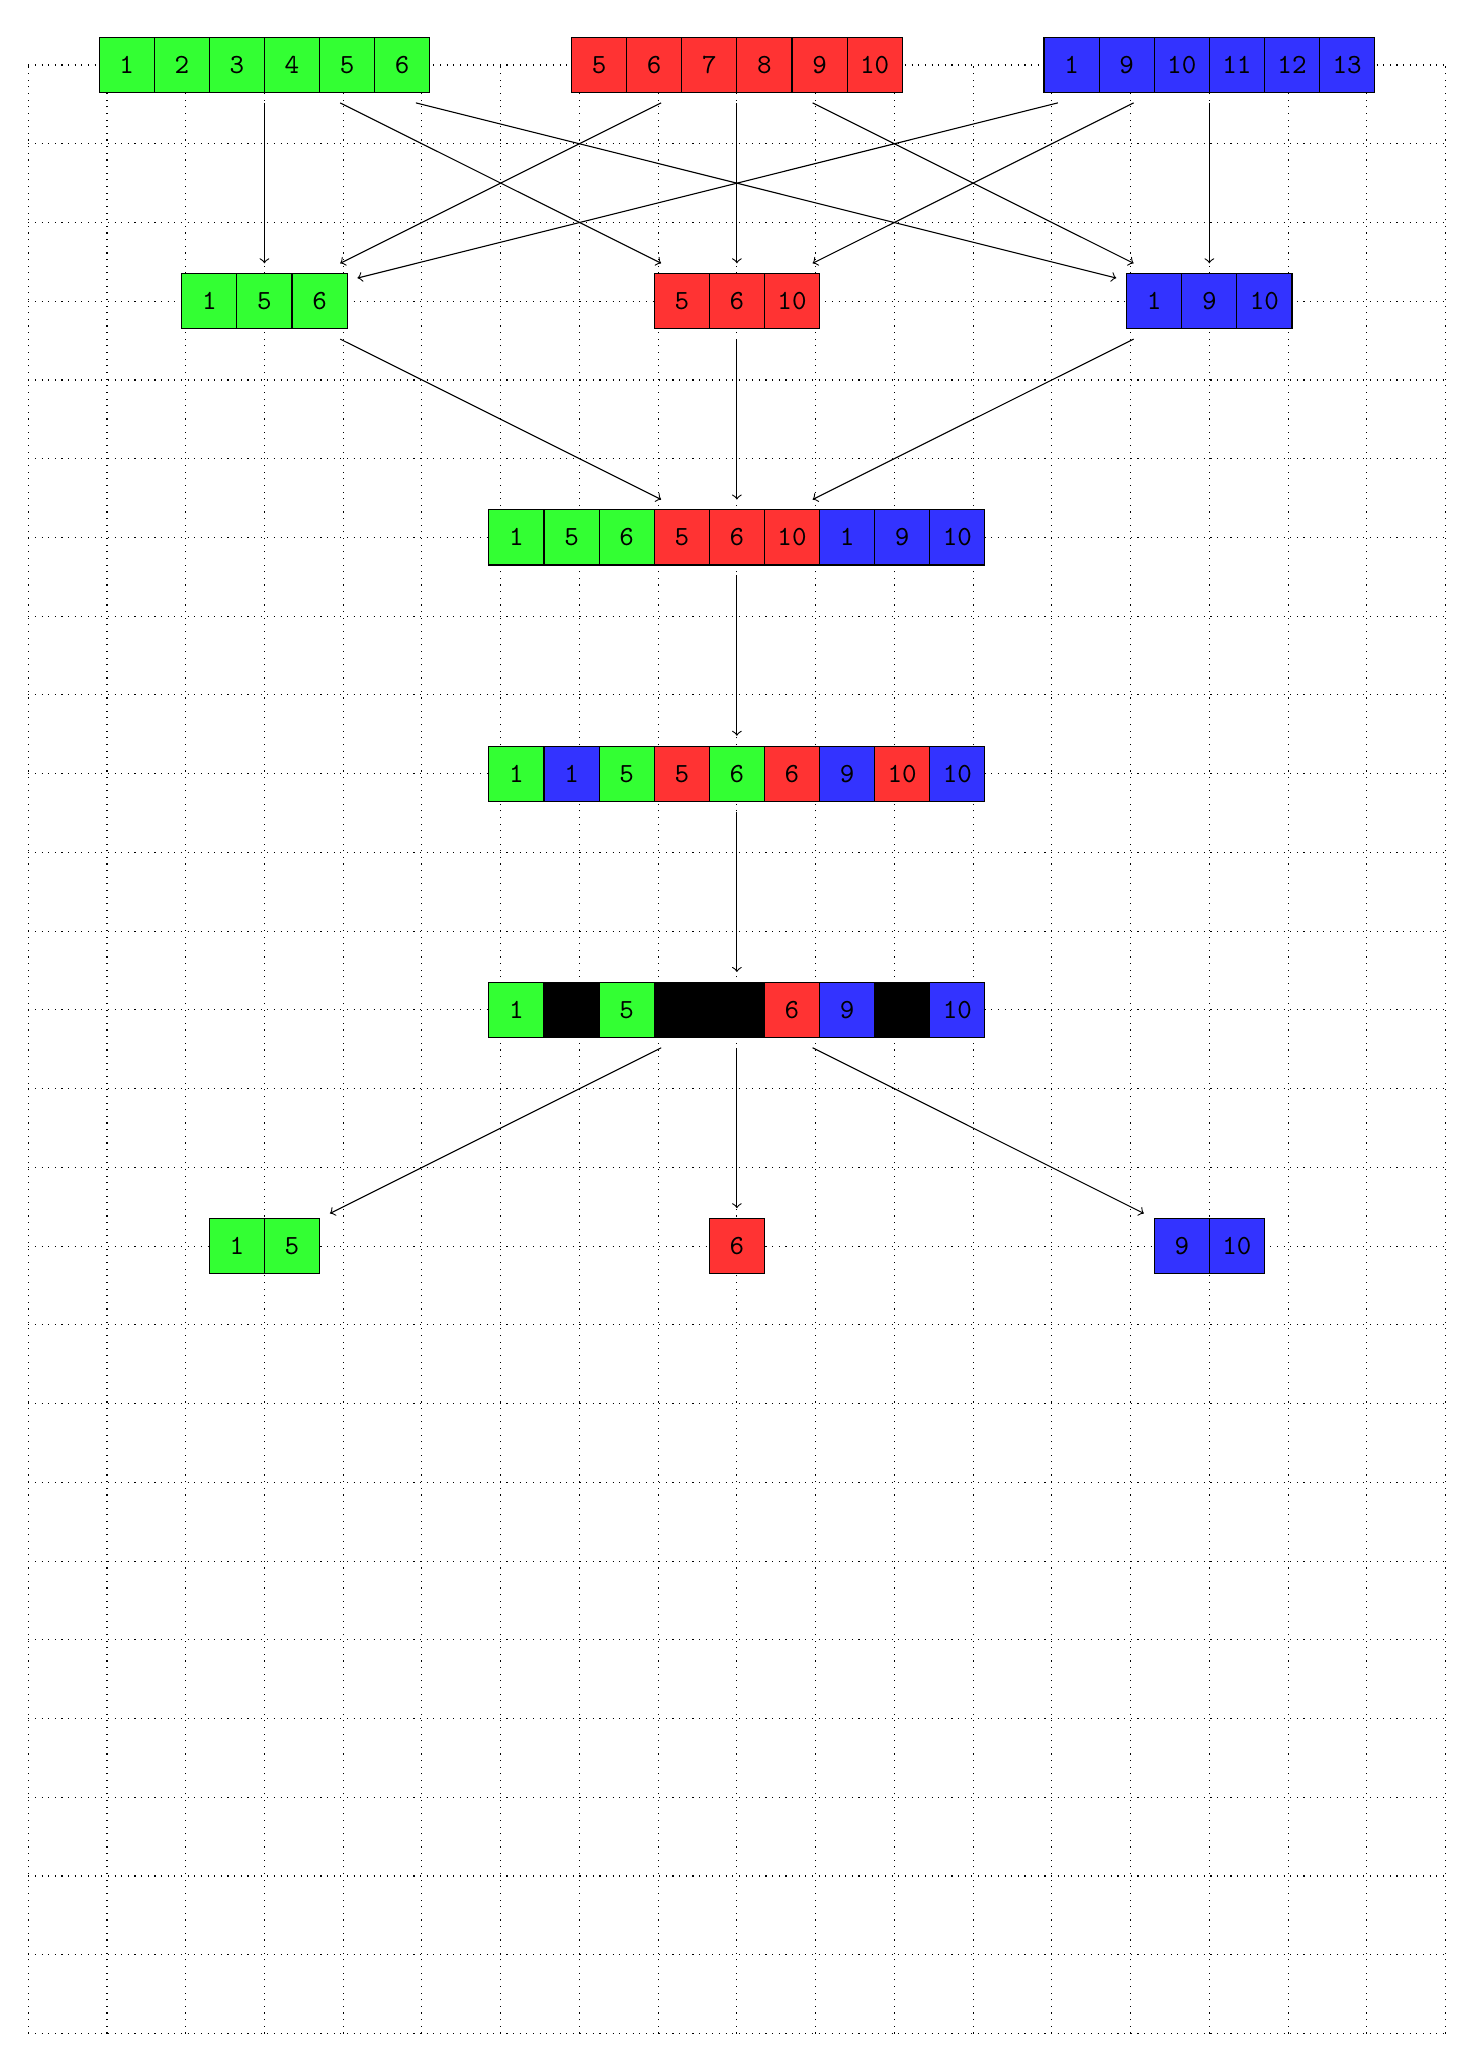
\begin{tikzpicture}[font=\ttfamily,
array_g/.style={matrix of nodes,nodes={draw, minimum size=7mm, fill=green!80},column sep=-\pgflinewidth, row sep=0.5mm, nodes in empty cells,
row 0/.style={nodes={draw=none, fill=none, minimum size=5mm}},
row 0 column 1/.style={nodes={draw}}},
array_r/.style={matrix of nodes,nodes={draw, minimum size=7mm, fill=red!80},column sep=-\pgflinewidth, row sep=0.5mm, nodes in empty cells,
row 0/.style={nodes={draw=none, fill=none, minimum size=5mm}},
row 0 column 1/.style={nodes={draw}}},
array_c/.style={matrix of nodes,nodes={draw, minimum size=7mm, fill=red!100},column sep=-\pgflinewidth, row sep=0.5mm, nodes in empty cells,
row 1 column 1/.style={nodes={draw, fill=green!80}},
row 1 column 2/.style={nodes={draw, fill=green!80}},
row 1 column 3/.style={nodes={draw, fill=green!80}},
row 1 column 4/.style={nodes={draw, fill=red!80}},
row 1 column 5/.style={nodes={draw, fill=red!80}},
row 1 column 6/.style={nodes={draw, fill=red!80}},
row 1 column 7/.style={nodes={draw, fill=blue!80}},
row 1 column 8/.style={nodes={draw, fill=blue!80}},
row 1 column 9/.style={nodes={draw, fill=blue!80}}
},
array_d/.style={matrix of nodes,nodes={draw, minimum size=7mm, fill=red!100},column sep=-\pgflinewidth, row sep=0.5mm, nodes in empty cells,
row 1 column 1/.style={nodes={draw, fill=green!80}},
row 1 column 2/.style={nodes={draw, fill=blue!80}},
row 1 column 3/.style={nodes={draw, fill=green!80}},
row 1 column 4/.style={nodes={draw, fill=red!80}},
row 1 column 5/.style={nodes={draw, fill=green!80}},
row 1 column 6/.style={nodes={draw, fill=red!80}},
row 1 column 7/.style={nodes={draw, fill=blue!80}},
row 1 column 8/.style={nodes={draw, fill=red!80}},
row 1 column 9/.style={nodes={draw, fill=blue!80}}
},
array_d/.style={matrix of nodes,nodes={draw, minimum size=7mm, fill=red!100},column sep=-\pgflinewidth, row sep=0.5mm, nodes in empty cells,
row 1 column 1/.style={nodes={draw, fill=green!80}},
row 1 column 2/.style={nodes={draw, fill=blue!80}},
row 1 column 3/.style={nodes={draw, fill=green!80}},
row 1 column 4/.style={nodes={draw, fill=red!80}},
row 1 column 5/.style={nodes={draw, fill=green!80}},
row 1 column 6/.style={nodes={draw, fill=red!80}},
row 1 column 7/.style={nodes={draw, fill=blue!80}},
row 1 column 8/.style={nodes={draw, fill=red!80}},
row 1 column 9/.style={nodes={draw, fill=blue!80}}
},
array_e/.style={matrix of nodes,nodes={draw, minimum size=7mm, fill=red!100},column sep=-\pgflinewidth, row sep=0.5mm, nodes in empty cells,
row 1 column 1/.style={nodes={draw, fill=green!80}},
row 1 column 2/.style={nodes={draw, fill=black!100}},
row 1 column 3/.style={nodes={draw, fill=green!80}},
row 1 column 4/.style={nodes={draw, fill=black!100}},
row 1 column 5/.style={nodes={draw, fill=black!100}},
row 1 column 6/.style={nodes={draw, fill=red!80}},
row 1 column 7/.style={nodes={draw, fill=blue!80}},
row 1 column 8/.style={nodes={draw, fill=black!100}},
row 1 column 9/.style={nodes={draw, fill=blue!80}}
},
array_b/.style={matrix of nodes,nodes={draw, minimum size=7mm, fill=blue!80},column sep=-\pgflinewidth, row sep=0.5mm, nodes in empty cells,
row 0/.style={nodes={draw=none, fill=none, minimum size=5mm}},
row 0 column 1/.style={nodes={draw}}}]

   \tikzstyle{state} =[fill=red,draw=none,text=white,minimum size=0.1cm]
   \tikzstyle{type2}=[fill=green,draw=none,text=white,minimum size=0.1cm]
   \tikzstyle{type3}=[fill=blue,draw=none,text=white,minimum size=0.1cm]

   % draw a grid for positioning nodes
   \coordinate (bottom_left) at (0,0);
   \coordinate (top_right) at (18,25);
   \draw [dotted, draw=black, fill=white] (bottom_left) grid  (top_right);

    \matrix[array_g] at (3,25) (A0) {
        1 & 2 & 3 & 4 & 5 & 6\\};
    \matrix[array_r] at (9,25) (A1) {
        5 & 6 & 7 & 8 & 9 & 10\\};
    \matrix[array_b] at (15,25) (A2) {
        1 & 9 & 10 & 11 & 12 & 13 \\};
    %\node[draw, fill=gray, minimum size=4mm] at (array-2-9) (box) {};

    \matrix[array_g] at (3,22) (B0) {
        1 & 5 & 6 \\};
    \matrix[array_r] at (9,22) (B1) {
        5 & 6 & 10 \\};
    \matrix[array_b] at (15,22) (B2) {
        1 & 9 & 10\\};

    \path [->] (A0) edge node {} (B0)
               (A1) edge node {} (B0)
               (A2) edge node {} (B0);

    \path [->] (A0) edge node {} (B1)
               (A1) edge node {} (B1)
               (A2) edge node {} (B1);

    \path [->] (A0) edge node {} (B2)
               (A1) edge node {} (B2)
               (A2) edge node {} (B2);

    \matrix[array_c] at (9,19) (C0) {
        1 & 5 & 6 & 5 & 6 & 10 & 1 & 9 & 10  \\};

    \path [->] (B0) edge node {} (C0)
               (B1) edge node {} (C0)
               (B2) edge node {} (C0);

    \matrix[array_d] at (9,16) (D0) {
        1 & 1 & 5 & 5 & 6 & 6 & 9 & 10 & 10  \\};

    \path [->] (C0) edge node {} (D0);

    \matrix[array_e] at (9,13) (E0) {
        1 & 1 & 5 & 5 & 6 & 6 & 9 & 10 & 10  \\};

    \path [->] (D0) edge node {} (E0);

    \matrix[array_g] at (3,10) (F0) {
        1 & 5 \\};
    \matrix[array_r] at (9,10) (F1) {
        6  \\};
    \matrix[array_b] at (15,10) (F2) {
        9 & 10 \\};

    \path [->] (E0) edge node {} (F0)
               (E0) edge node {} (F1)
               (E0) edge node {} (F2);

\end{tikzpicture}

\end{document}



%%%%%%%%%%%%%%%%%%%%%%%%%%%%%%%%%%%%%%%%%%%%%%%%%%%%%%%%%%%%%

\begin{forest}
   for tree={
             font=\ttfamily,
             grow'=0,
             child anchor=west,
             parent anchor=south,
             anchor=west,
             calign=first,
             edge path={
                          \noexpand\path [draw, \forestoption{edge}]
                            (!u.south west) +(7.0pt,0) |- node[fill,inner sep=1.20pt] {} (.child
                                anchor)\forestoption{edge label};
                        },
             before typesetting nodes={
             if n=1
             {insert before={[,phantom]}}
             {}
             },
             fit=band,
             before computing
               xy={l=12pt},
             }
[sputnik
[src
[spu_parser.c]
[list.c]
]
[macro
[src
[mac_parser.c]
[mac_color.c]
[mac_mesh.c]
]
[inc
[macro.h]
]
]
[micro
[src
[mic_parser.c]
[mic_color.c]
[mic_mesh.c]
]
[inc
[micro.h]
]
]
]
\end{forest}


\chapter*{Fermi Input Manual}

%%%%%%%%%%%%%%%%%%%%%%%%%%%%%%%%%%%%%%%%%%%%%%%%%%%%%%%%%%%%%%%%%%%%%%%%%%%%%%%%%%%%

\definecolor{mygreen}{rgb}{0.3, 0.9, 0.1}

%%%%%%%%%%%%%%%%%%%%%%%%%%%%%%%%%%%%%%%%%%%%%%%%%%%%%%%%%%%%%%%%%%%%%%%%%%%%%%%%%%%

\section{Input file}

\subsection{Mesh information}

\begin{Verbatim}[frame=single,commandchars=\\\{\}]

\textcolor{Green}{# MACRO INFORMATION}
\textcolor{Green}{# <# PROCESSES> }
    2  
\textcolor{Green}{# MICRO INFORMATION}
\textcolor{Green}{# <# PROCESSES> }
    6  
\textcolor{Green}{# <#KINDS> }
    3
\textcolor{Green}{# <# PROCESSES KIND 0> <# PROCESSES KIND 1> <# PROCESSES KIND 2>}
    1                    1                    1
\end{Verbatim}


%%%%%%%%%%%%%%%%%%%%%%%%%%%%%%%%%%%%%%%%%%%%%%%%%%%%%%%%%%%%%%%%%%%%%%%%%%%%%%%%%%%%


%\begin{alltt}
%<nXSf> = <  \(\nu\sigma_{1}^{f}\) \(\nu\sigma_{2}^{f} \dots \nu\sigma_{g}^{f}\) > 
%\end{alltt}


\chapter*{\micro}

\section{Introduction}

The \micro was designed to calculate the average properties on micro-structures. 
It uses ParMETIS and PETSc libraries to partition the domain and solving the equilibrium problem in parallel.

This code uses the main \sputnik routines for the mesh treatment and assembly operations and it design in a very
minimalistic way focusing on achieve high performance retrieving fast as possible The homogenized values.

\section{Methods}

The code can operate in \emph{coupling} or \emph{standalone} mode. The \emph{coupling} will generally be used to
perform multi-scale calculations coupling \macro with \micro as:

\begin{lstlisting}[frame=single,language=bash]
<@\textcolor{blue}{mpirun}@> -np <np_M> <@\textcolor{OliveGreen}{macro}@> -coupl [OPTIONS_M] : -np <np_m> <@\textcolor{OliveGreen}{micro}@> -coupl [OPTIONS_m]
\end{lstlisting}

Notice the using of the \verb -coupl option.

\begin{lstlisting}[frame=single,language=bash]
<@\textcolor{blue}{mpirun}@> -np <np_m> <@\textcolor{OliveGreen}{micro}@> [OPTIONS_m]
\end{lstlisting}

\section{The coupling execution}

\section{The standalone execution}


\bibliography{sputnik}{}
\bibliographystyle{plain}
%%%%%%%%%%%%%%%%%%%%%%%%%%%%%%%%%%%%%%%%%%%%%%%%%%%%%%%
% Sample table                                        %
% Source: www1.maths.leeds.ac.uk/latex/TableHelp1.pdf %
%%%%%%%%%%%%%%%%%%%%%%%%%%%%%%%%%%%%%%%%%%%%%%%%%%%%%%%
% \begin{table}[ht]
% \caption{Sample table} % title of Table
% \centering % used for centering table
% \begin{tabular}{c c c c}
% % centered columns (4 columns)
% \hline\hline %inserts double horizontal lines
% S. No. & Column\#1 & Column\#2 & Column\#3 \\ [0.5ex]
% % inserts table
% %heading
% \hline % inserts single horizontal line
% 1 & 50 & 837 & 970 \\
% 2 & 47 & 877 & 230 \\
% 3 & 31 & 25 & 415 \\
% 4 & 35 & 144 & 2356 \\
% 5 & 45 & 300 & 556 \\ [1ex] % [1ex] adds vertical space
% \hline %inserts single line
% \end{tabular}
% \label{table:nonlin} % is used to refer this table in the text
% \end{table}

% Duis aute irure dolor in reprehenderit in voluptate velit esse cillum dolore eu fugiat nulla pariatur. Excepteur sint occaecat cupidatat non proident, sunt in culpa qui officia deserunt mollit anim id est laborum. \\ Lorem ipsum list:
% \begin{itemize}
% \item Mauris sit amet nulla mi, vitae rutrum ante.
% \item Maecenas quis nulla risus, vel tincidunt ligula.
% \item Nullam ac enim neque, non \emph{dapibus} mauris.
% \end{itemize}
% 
% \noindent Lorem ipsum dolor sit amet, consectetur adipiscing elit. Duis risus ante, auctor et pulvinar non, posuere ac lacus. Praesent egestas nisi id metus rhoncus ac lobortis sem hendrerit. Etiam et sapien eget lectus interdum posuere sit amet ac urna\footnote{Lorem ipsum dolor sit amet, consectetur adipiscing elit. Duis risus ante, auctor et pulvinar non, posuere ac lacus.}:
% 
% \subsection{Lorem ipsum dolor sit amet, consectetur adipiscing elit.}
% Lorem ipsum dolor sit amet, consectetur adipiscing elit. Duis risus ante, auctor et pulvinar non, posuere ac lacus. Praesent egestas nisi id metus rhoncus ac lobortis sem hendrerit. Etiam et sapien eget lectus interdum posuere sit amet ac urna. Aliquam pellentesque imperdiet erat, eget consectetur felis malesuada quis. Pellentesque sollicitudin, odio sed dapibus eleifend, magna sem luctus turpis, id aliquam felis dolor eu diam. Etiam ullamcorper, nunc a accumsan adipiscing, turpis odio bibendum erat, id convallis magna eros nec metus. Sed vel ligula justo, sit amet vestibulum dolor. Sed vitae augue sit amet magna ullamcorper suscipit. Quisque dictum ipsum a sapien egestas facilisis. 
% 
% \subsection{Lorem ipsum dolor sit amet, consectetur adipiscing}
% Lorem ipsum dolor sit amet, consectetur adipiscing elit. Duis risus ante, auctor et pulvinar non, posuere ac lacus. Praesent egestas nisi id metus rhoncus ac lobortis sem hendrerit. Etiam et sapien eget lectus interdum posuere sit amet ac urna. Aliquam pellentesque imperdiet erat, eget consectetur felis malesuada quis. Pellentesque sollicitudin, odio sed dapibus eleifend, magna sem luctus turpis, id aliquam felis dolor eu diam.

\end{document}
